\documentclass[11pt]{article}
\usepackage[margin=1in]{geometry}
\usepackage{graphicx}
\usepackage{amsmath}
\usepackage{amssymb}
\usepackage{float}
\usepackage{subcaption}

\title{June 10, 2021 Meeting Agenda}

\begin{document}
\maketitle

\section{Joint estimation of $\mu_p$ and $\mu_t$}
This week I worked on implementing the plots we talked about last time. One of them is a plot of
the negative log likelihood vs $\mu_p$. The other is Nasser's plot of number of trials vs $\mu_t$.
The graphs are shown below. I also added a table with the progression of $\mu_t$ and $\mu_p$ throughout the course of the algorithm. I caught a mistake in how I was calculating $\mu_t$ and I've fixed it. Our current estimate of $\mu_t = 0.081$ which is about 12 days per trial. Our current estimate of $\mu_p = 13.19$.

\begin{figure}[H]
  \centering
    \begin{subfigure}[b]{0.45\textwidth}
      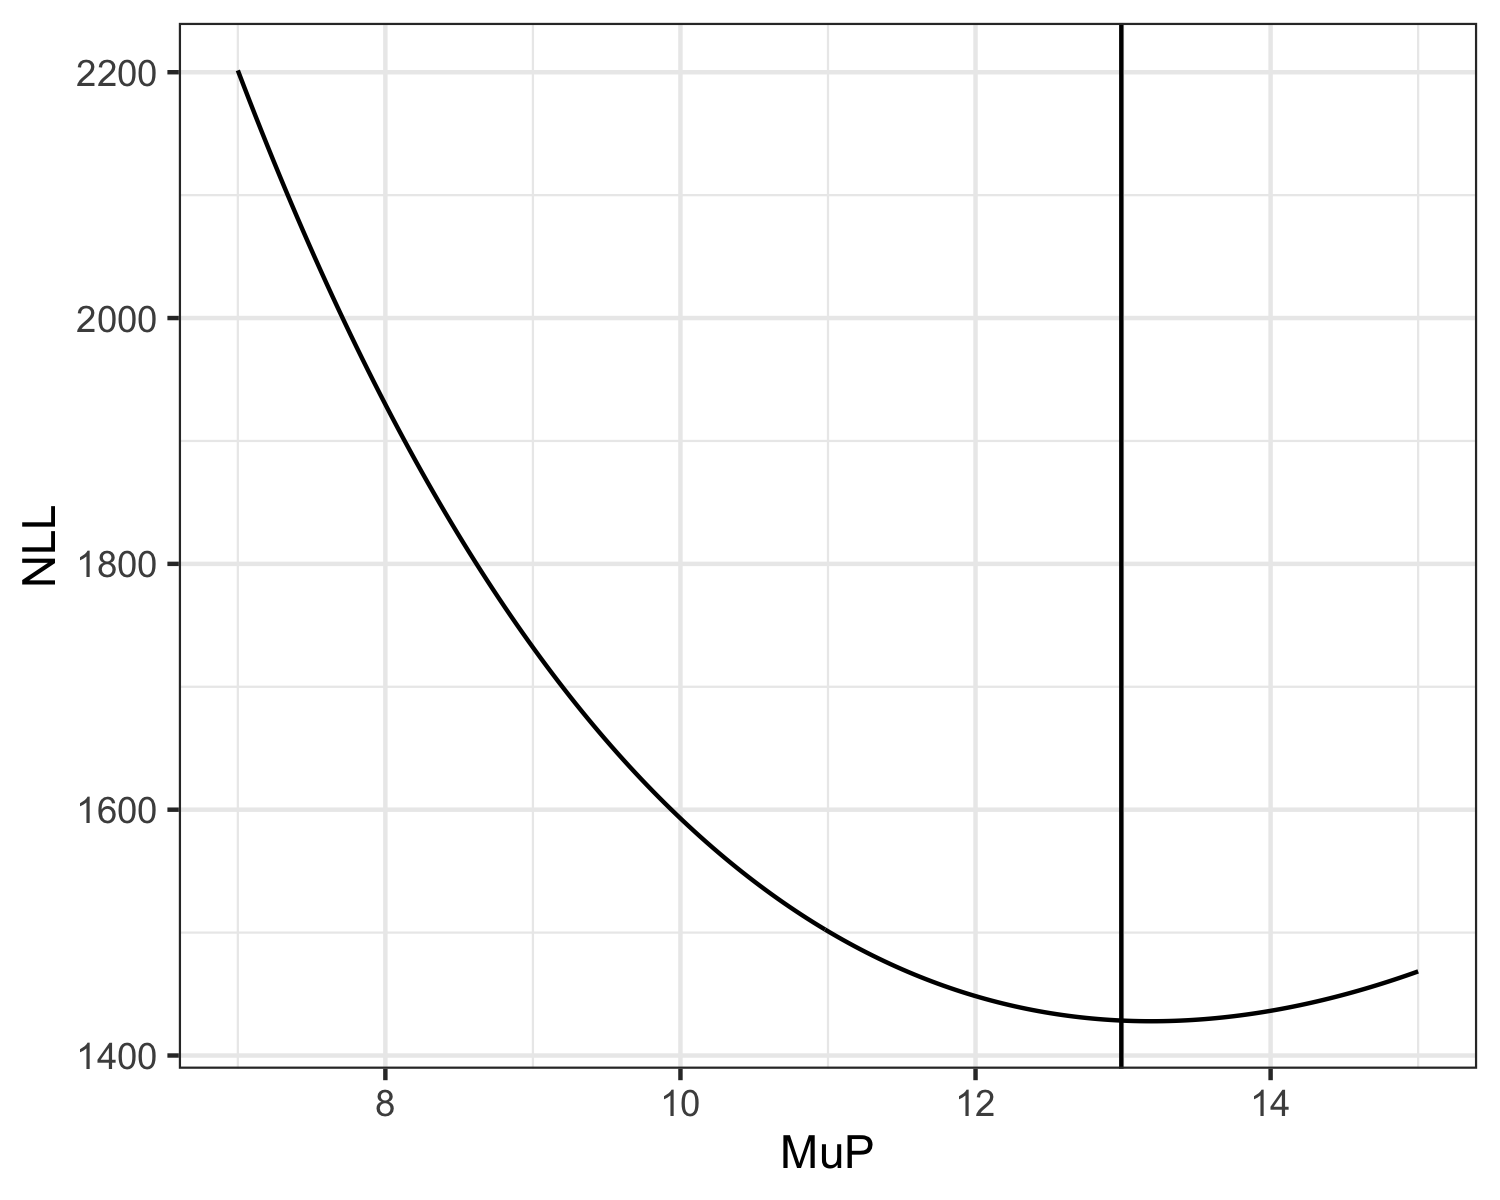
\includegraphics[width=\textwidth]{../../../output/figures/Optimization/opt_data_0.png}
      \caption{Iteration 1}
      \label{fig:f1}
    \end{subfigure}
    \hfill
    \begin{subfigure}[b]{0.45\textwidth}
      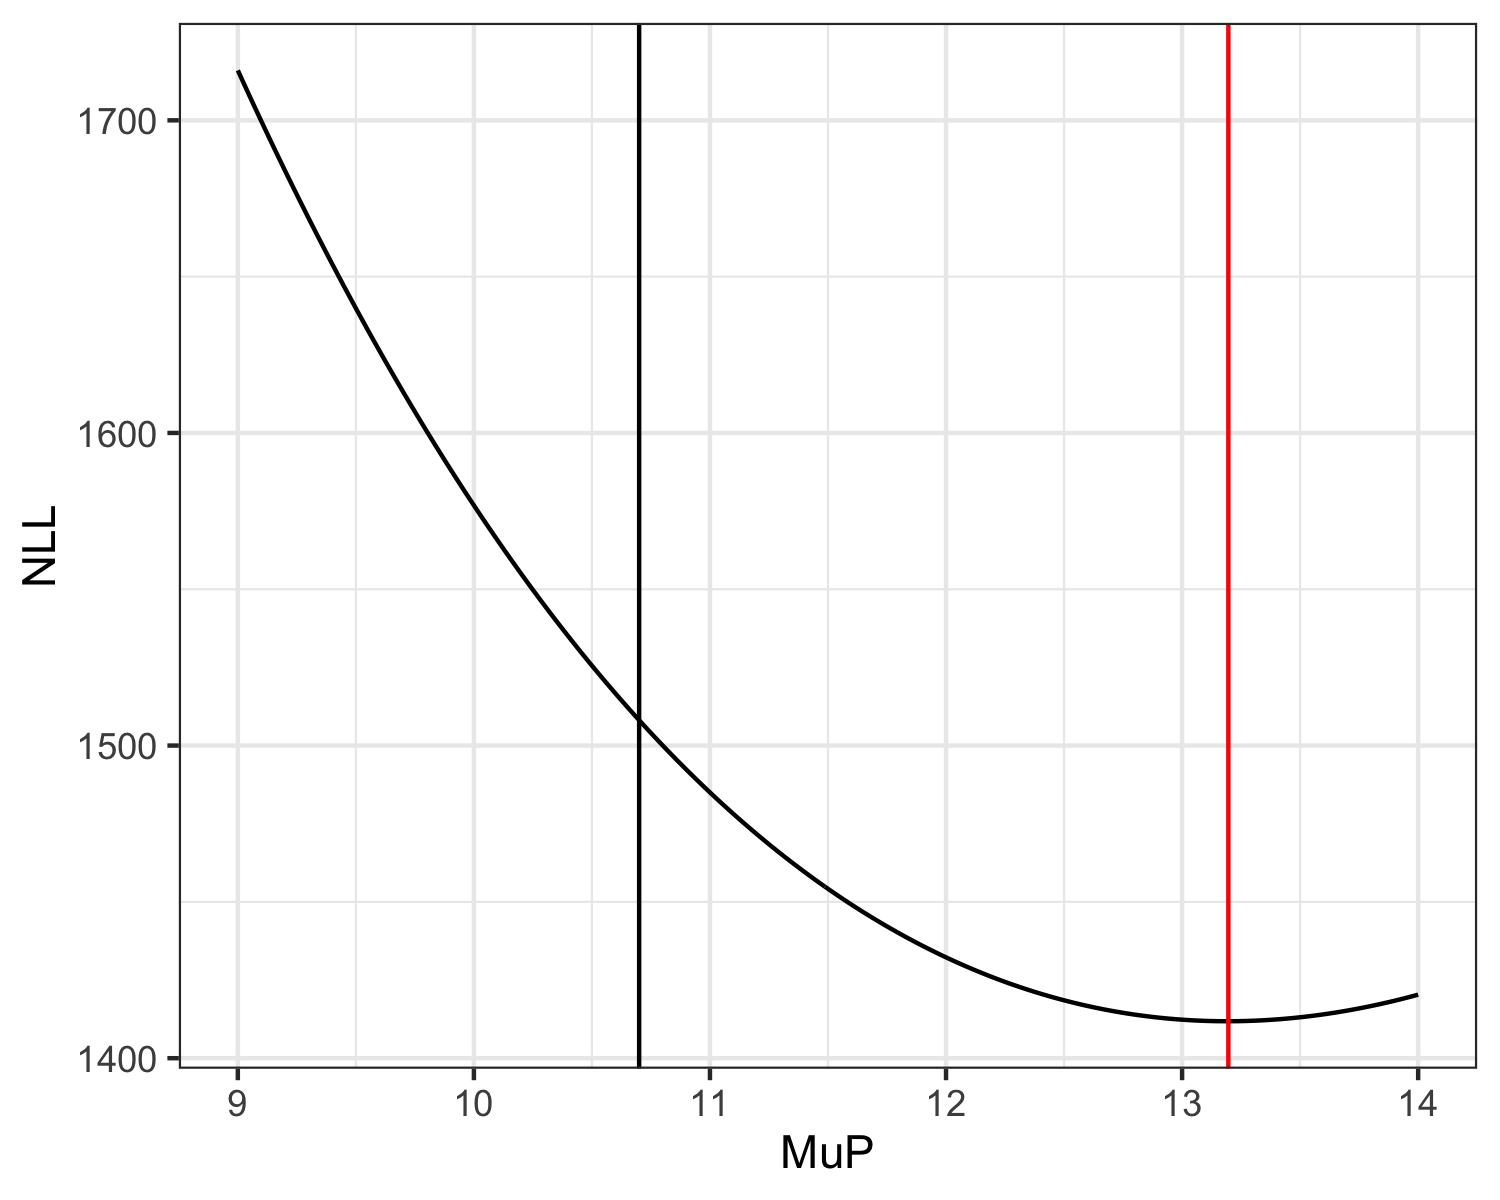
\includegraphics[width=\textwidth]{../../../output/figures/Optimization/opt_data_1.png}
      \caption{Iteration 2}

    \end{subfigure}
    %\hfill
    \begin{subfigure}[b]{0.45\textwidth}

      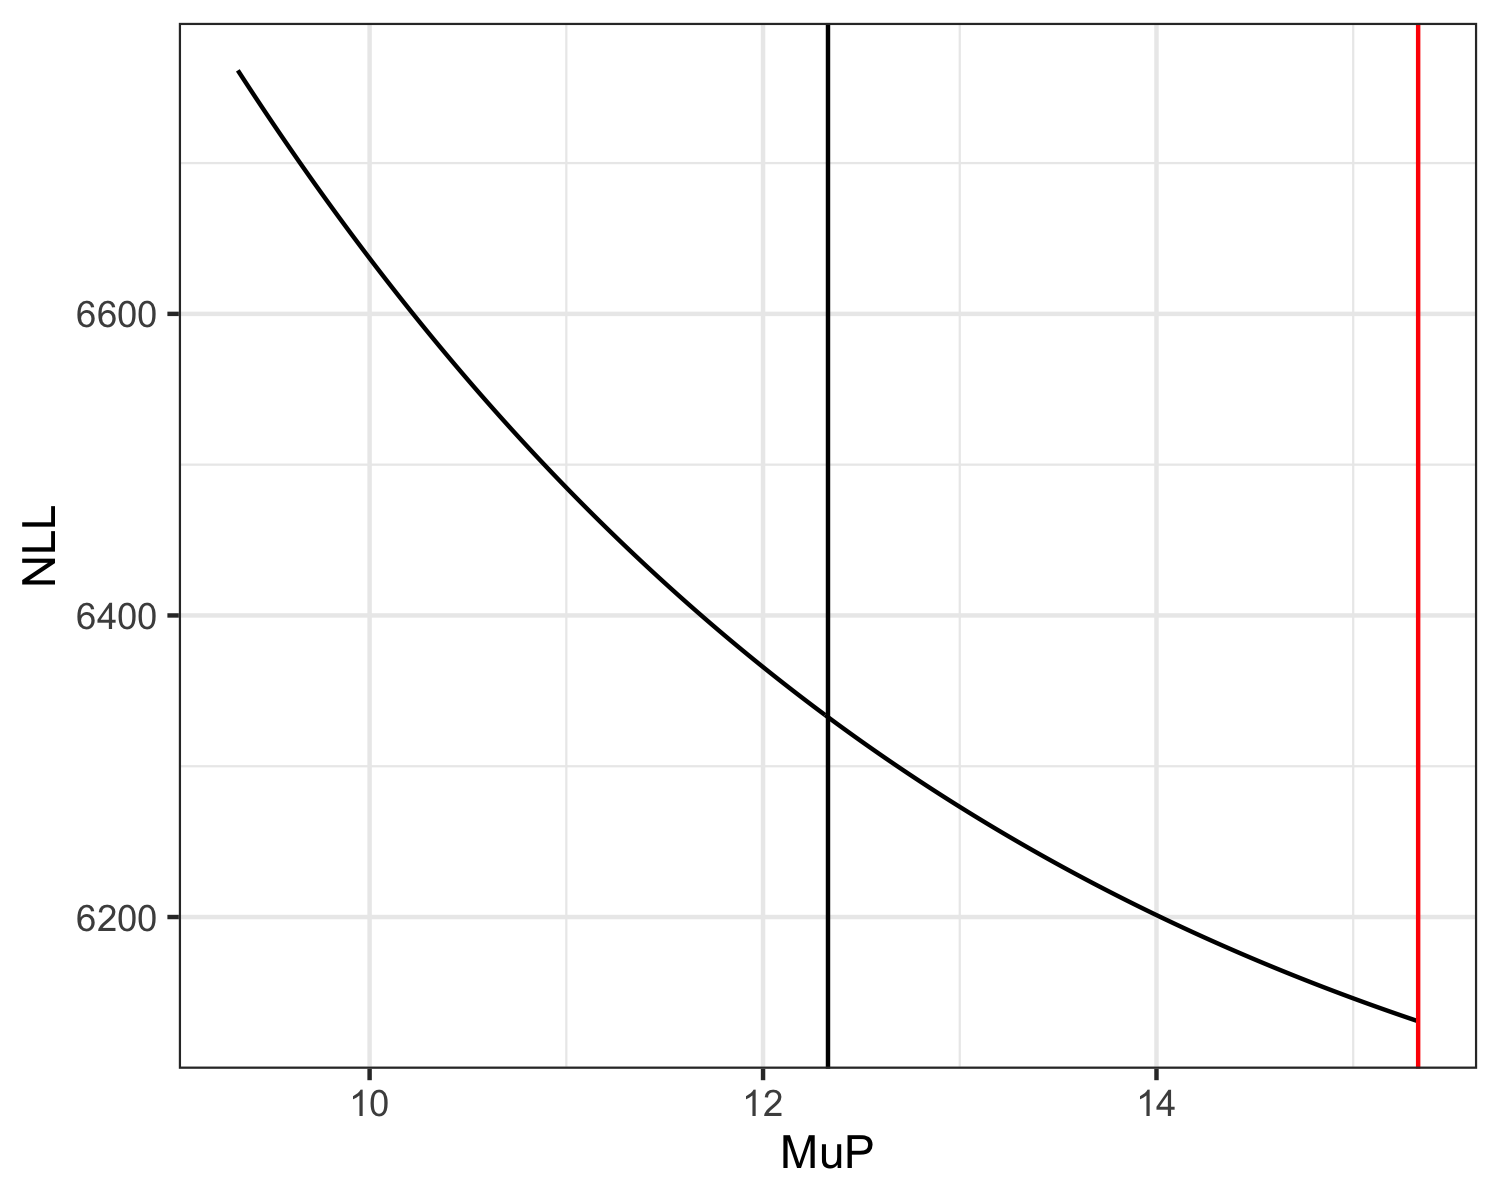
\includegraphics[width=\textwidth]{../../../output/figures/Optimization/opt_data_2.png}
      \caption{Iteration 3}

    \end{subfigure}
    \caption{Negative log likelihood vs $\mu_p$}
\end{figure}

\begin{figure}[H]
  \centering
    \begin{subfigure}[b]{0.45\textwidth}
      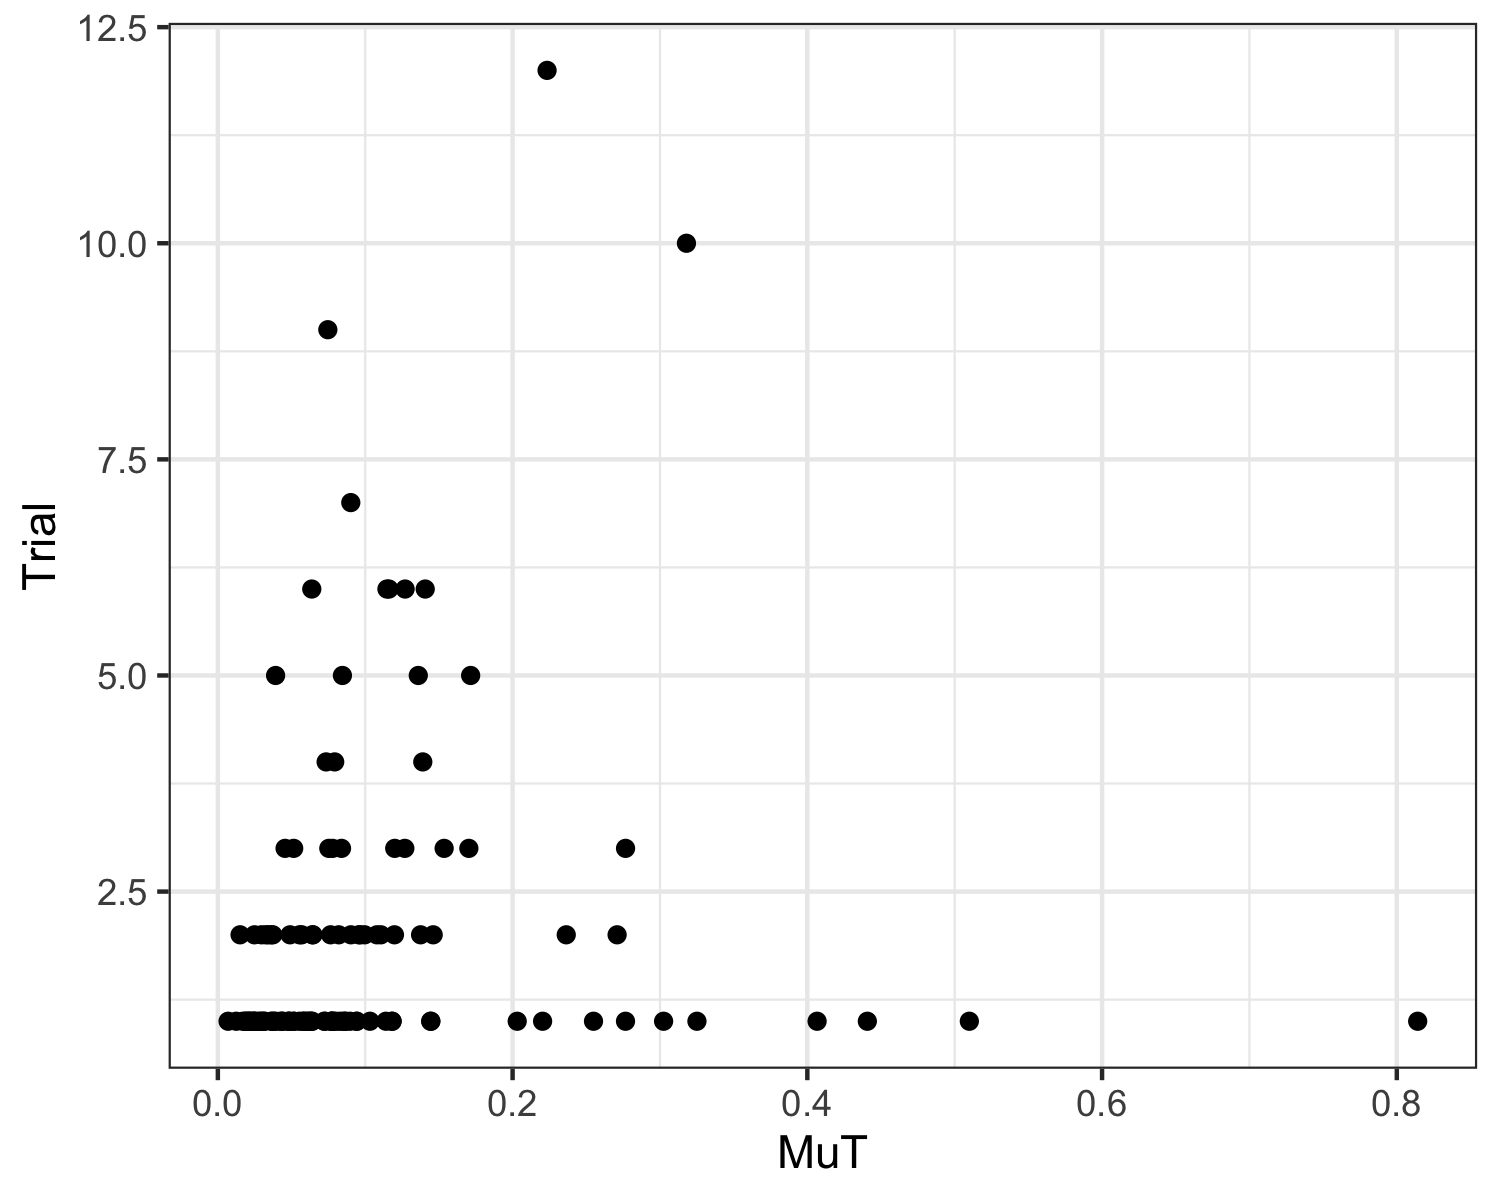
\includegraphics[width=\textwidth]{../../../output/figures/Optimization/mut_data_0.png}
      \caption{Iteration 1}
      \label{fig:f1}
    \end{subfigure}
    \hfill
    \begin{subfigure}[b]{0.45\textwidth}
      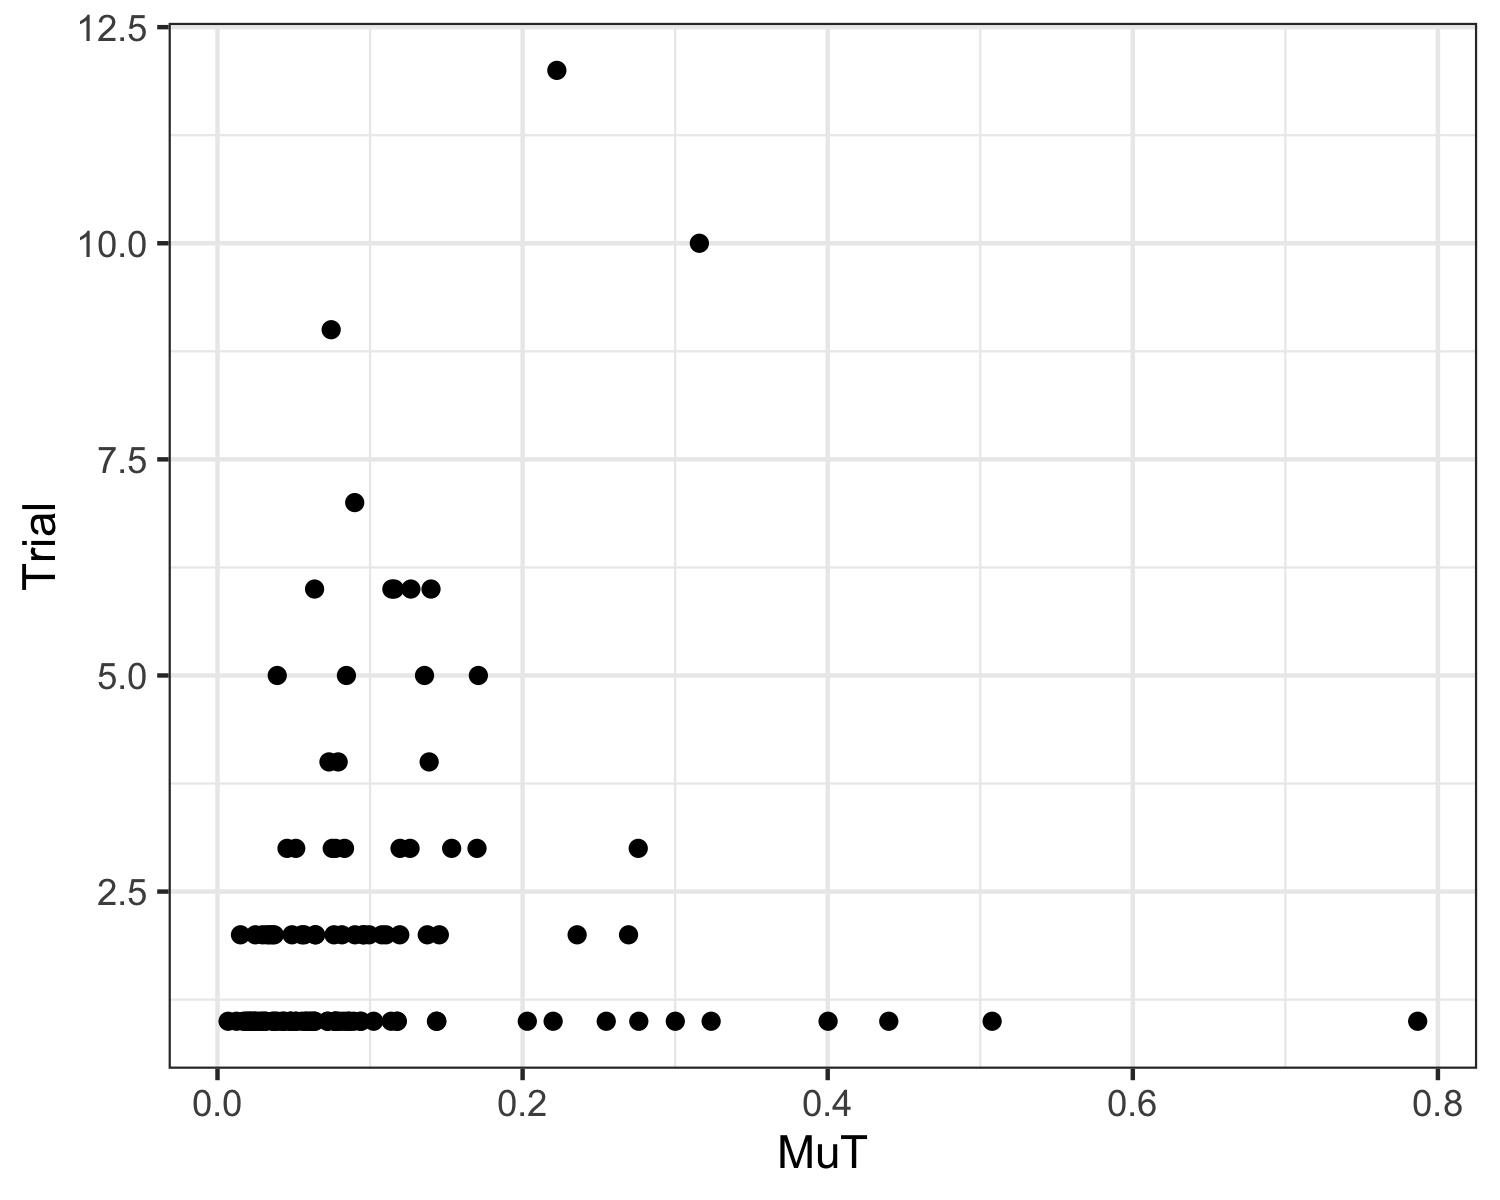
\includegraphics[width=\textwidth]{../../../output/figures/Optimization/mut_data_1.png}
      \caption{Iteration 2}

    \end{subfigure}
    %\hfill
    \begin{subfigure}[b]{0.45\textwidth}

      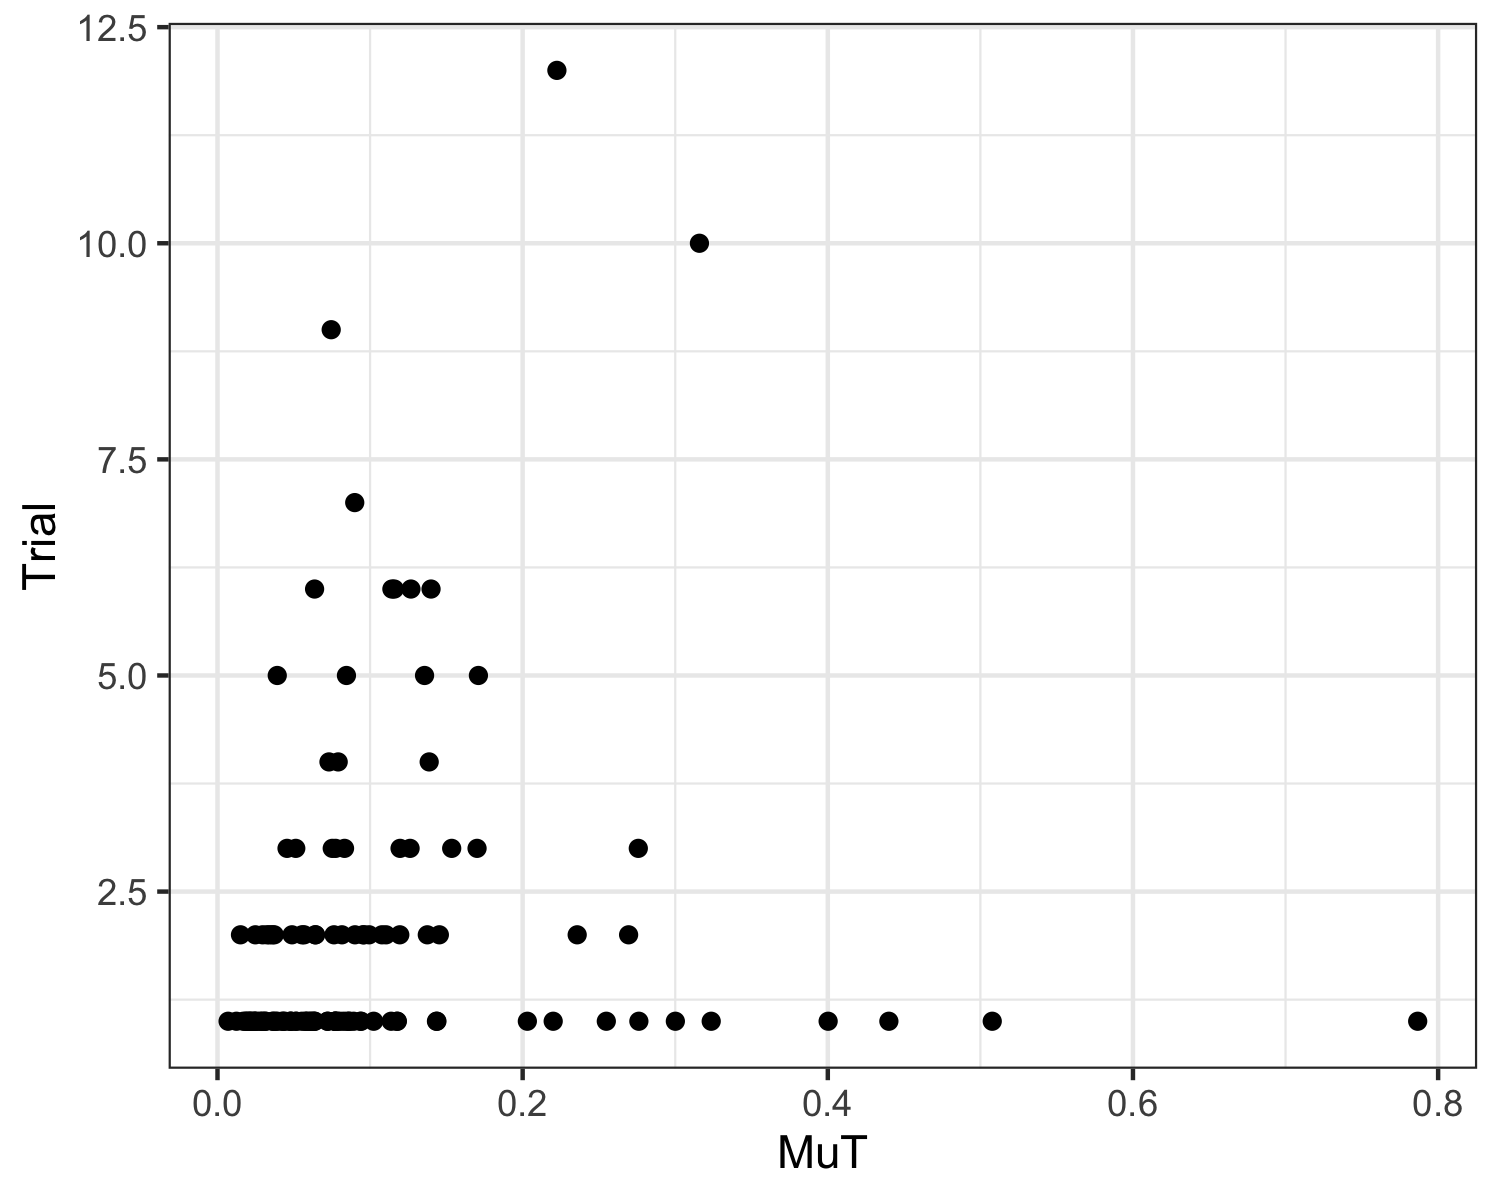
\includegraphics[width=\textwidth]{../../../output/figures/Optimization/mut_data_2.png}
      \caption{Iteration 3}

    \end{subfigure}
    \caption{Number of Trials vs $mu_t$}
\end{figure}

\begin{table}[H]
  \centering
  \caption{Evolution of $\mu_p$ and $\mu_t$}
  \label{tab:my-table}
  \begin{tabular}{|l|l|l|}
  \hline
  \textbf{Iteration} & \textbf{$\mu_t$} & \textbf{$\mu_p$} \\ \hline
  0                  & 0.12         & 10.7         \\ \hline
  1                  & 0.082        & 12.99        \\ \hline
  2                  & 0.081        & 13.19        \\ \hline
  3                  & 0.081        & 13.19        \\ \hline
  \end{tabular}
\end{table}


  \subsection{Next Steps}
  \begin{itemize}
    \item Do Poisson tail calculations.
    \item Add information about optimizer to document.
  \end{itemize}

\end{document}
